% Recharge : de 2 à au moins 8 unités
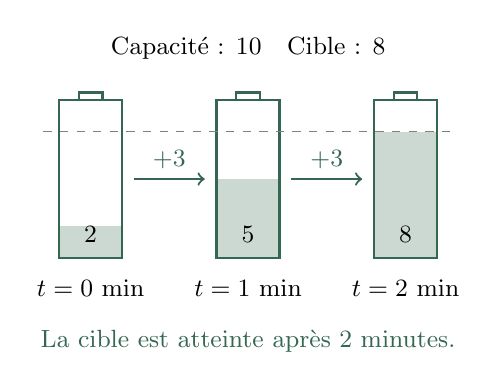
\begin{tikzpicture}[x=1cm,y=1cm,font=\small]
\definecolor{vert}{RGB}{53,102,81}
\foreach \x/\niveau/\temps in {0/2/0,2/5/1,4/8/2} {
  \fill[vert!25] (\x,0) rectangle (\x+0.8,\niveau/5);
  \draw[thick,vert] (\x,0) rectangle (\x+0.8,2);
  \draw[thick,vert] (\x+0.25,2) -- (\x+0.25,2.1) -- (\x+0.55,2.1) -- (\x+0.55,2);
  \node at (\x+0.4,0.3) {$\niveau$};
  \node[below] at (\x+0.4,-0.15) {$t=\temps$ min};
}
\draw[->,thick,vert] (0.95,1) -- (1.85,1) node[midway,above] {$+3$};
\draw[->,thick,vert] (2.95,1) -- (3.85,1) node[midway,above] {$+3$};
\draw[dashed,gray] (-0.2,1.6) -- (5,1.6);
\node[above,align=center] at (2.4,2.4) {Capacit\'e : 10\quad Cible : 8};
\node[below,text=vert] at (2.4,-0.8) {La cible est atteinte apr\`es 2 minutes.};
\end{tikzpicture}
